% We have designed a test based on previous tests of response systems with the purpose of finding out if the systems is able to increase interaction in class. The test and the design of the test will be described in detail in this section.

\section{Testing CRSFIT in a classroom}\label{sec:testingcrs}
%The following sections will describe the methods we will use to test CRSFIT and the analysis of our results.
We have designed a test in order to tell whether or not our solution can have a positive impact on teaching classes that covers teaching programming and mathematics. The test is inspired by \cite{siau2006use} and their work. \citeA{siau2006use} found that there wasn't developed any instrument for measuring interactivity. This resulted in \citeA{siau2006use} to create their own method, from which we have taken elements to support our own.

The following sections will also include the analysis of the results from our questionnaires. With students from two different courses participating in our test, we will compare the results from each course using CRSFIT in one, and a different system in the other. Qualitative results from our questionnaires will be examined in order to discover areas of the test and system which could be improved.


\subsection{Measuring interactivity}
The test by \citeA{siau2006use} is designed to tell whether or not they are able to move peoples behaviour, beliefs and attitude towards engagement, interactivity and participation during class. The test they designed consists of a \emph{pretest}, \emph{implementation} (of the system in a class) and a \emph{posttest} followed up by a \emph{qualitative data collection}. The pretest and posttest were made as questionnaires and the implementation was a hardware based CRS solution.

Our test is structured in the same way and we are asking similar questions in the different parts of the test as well. The whole test should preferably be carried out over a whole semester, but due to the limited time of this project the tests will be carried out in a single lecture in two different courses. The courses used in our tests was \emph{Frameworks and Architectures for the Web} and \emph{Advanced Programming}.

By having a pretest and a posttest asking the same questions \citeA{siau2006use} was able to compare the results and measure whether or not they were able to move peoples attitude. Their pretest consisted of two parts which were asking about individual interactivity and general interactivity in the class. The questions in both parts of the pretest were formulated as statements such as \emph{"I am engaged in class"} and \emph{"I provide my opinion to questions from the teacher during the class"}. This part of their test will be almost identical to our test. Our test primarily differs from theirs in the posttest. Since we are not able to carry out our test over a longer period of time, our posttest will not be asking into \emph{individual interactivity} and \emph{general interactivity} again. We will, however, use the results from \emph{individual interactivity} and \emph{general interactivity} from the pretest to tell to which degree students interact in class in general. The pretest should be answered by students before or in the beginning of the given lecture in which the test is carried out (See appendix \ref{app:pretest} for the complete list of questions from the pretest questionnaire).

During the lecture of the Frameworks course we asked students questions relevant to their class using our solution, CRSFIT. This part of the test is the \emph{implementation}. Students answered the questions anonymously and they were not held accountable. The purpose of this part of the test is to 1) tell if students actually benefit from using the system and overall find it useful, and 2) test our solution in a real setting.

It requires training and experience to get the most out of a classroom response system. The literature and insights about how to use response systems in a beneficial way has developed alongside with the research of the implementation of response system in classrooms. For example, see: \cite{lantz2014effectiveness,draper2004increasing,lin2011implementing} for insights and comments about how to effectively use response systems. 
We have developed questions for the Frameworks course in collaboration with our supervisor, Peter Eklund, which was asked during the lecture in which we carried out the test.
The questions that where asked during the test in the Frameworks course can be found in appendix \ref{app:questions} and on the live site at \url{http://crsfit.online/r/b4tc8} (login required). 

The questions asked in Advanced Programming, was developed by the course teacher, Andrzej Wasowski. The questions can be found in appendix \ref{app:questions-advanced}.


\subsection{Acceptance of technology}
In the posttest questionnaire we ask students about the perceived ease of use of CRSFIT and the perceived usefulness. The \emph{perceived ease of use} is included in the test in order to get feedback on how easy the system is to use. The \emph{perceived usefulness} asks into the idea and possible benefits of the system with statements like \emph{"Using the system makes it easier for me to interact in the class"} to be rated. Perceived ease of use and perceived usefulness is adopted from the \emph{Technology Acceptance Model (TAM)} \cite{siau2006use,davis1989user} where they are defined as follows:

\emph{"Perceived usefulness (U) is defined as the prospective user's subjective probability that using a specific application system will increase his or her job performance within an organizational context. Perceived ease of use (EOU) refers to the degree to which the prospective user expects the target system to be free of effort."} \cite[p.~985]{davis1989user}.

The model originally aims to predict users intention to adopt new technology. We will, however, not use the model as it was intended. Inspired by the questions in a different research project by \citeA{davis1989perceived} we will ask similar styled questions in our posttest.

This part of the test will tell if the students feel an individual increased interactivity by using our system. Also, we ask the students whether or not they use any tools to test their answers which includes any code/script or mathematical expressions. Included in the posttest questionnaire is also an open ended question in which we ask students to give their opinion about advantages and disadvantages of using a classroom response system. This is the qualitative part of the test. This part serves to give us an idea about areas that this kind of system does particular good or bad. See appendix \ref{app:posttest} for a complete list of the questions from the posttest questionnaire.


\subsection{The pretest and posttest questionnaires} % Field testing the system with quantitative and some qualitative data
% Likert scale
% Spørgsmål - se bog. Structured format (i form af at spørgsmålene ikke bliver spurgt af os, men står på tekst (spørgeskema). Likert skala, 1-9. (Find artikel)
% Open ended spørgsmål til at slutte af med - kvalitativ data som vi vil bruge til ?? i analysen.
The pretest and the posttest are designed as questionnaires. Questionnaires makes the least demands on personal and social skills of the questioner \cite[p.~74]{deacon2007researching} and enables us to measure the results. The questionnaires are to be answered online using Google Forms\footnote{\url{https://www.google.dk/intl/da/forms/about/}}. Our way of asking the questions are highly structured since they are written down (using Google Forms) and asked in the exact same way to all participants \cite[p.~65]{deacon2007researching}. Both questionnaires can be found in the appendix (\ref{app:pretest}, \ref{app:posttest}).

When asking questions in a questionnaire (or in general) the questioner should be aware which type of questions are asked. What does the question seek to find information about? \citeA[pp.~80-84]{dillman1978mail} lists four types of questions which are asking into either \emph{behaviour}, \emph{beliefs}, \emph{attitudes} or \emph{attributes}. With our questions we are interested in behaviour, beliefs and attitudes. We are not focusing on attributes. Questions asking into attributes are concerned about background information of the respondent such as age, gender etc. \cite[p.~75]{deacon2007researching}. While these questions typically are easy to answer, they are of no interest to us. They are often used to say something about a group of people you don't know and are of most use in very large samples. Our questions are interested in behaviour when we ask student to rate statements such as \emph{"I interact with the teacher in class"} and beliefs (\emph{"Students receive feedback from the teacher during the class"}) and attitudes (\emph{"I find the system useful in enhancing my interaction in the class"}).

It may seem that some of our questions are identical to each other even though they are slightly different. Because of this we risk that respondents doesn't see the difference from the previous question and therefore may answer the same as in the previous question. Because of the similarity we could risk that respondents find the questionnaire as a whole to be frustrating or difficult to answer.

All of the questions in our questionnaires (except two) are formulated as statements which should be answered on a Likert scale \cite{likert1932technique} with items 1-9 where 1 is \emph{Strongly disagree} and 9 is \emph{Strongly agree}. With an uneven number we offer a neutral choice (5 on our scale) in order to avoid forcing an opinion on the respondents. We could have chosen to make the scale smaller or larger. A smaller scale than 1-9 could result in less different answers since the options are fewer. \citeA[p.~507]{matell1972there} found that less than 7 options on a Likert scale resulted in greater usage of the "neutral" choice. In order to avoid that we choose 9 options which we hope will not offer too many options as well.


%To sum things up the following list shows what we'll do and when:

%\begin{itemize}
%    \item Pretest: Questionnaire, before or in the beginning of the lecture
%    \item Implementation: Students answer questions with CRSFIT during lecture
%    \item Posttest + qualitative data: Questionnaire, in the end of the lecture
%\end{itemize}

\subsection{Analysis of tests}

The two tests were carried out in a classroom setting in two different courses, \emph{Advanced Programming} (the Advanced course) and \emph{Frameworks and Architectures for the Web} (the Frameworks course). All students in each class were given the pretest and the posttest, and used a CRS system in between. The Advanced course used Mentimeter, and have done so throughout the semester. The Frameworks course used our system, CRSFIT, and have not used any other CRS throughout the semester.
There were 10 students present while performing the tests in the Frameworks course. This resulted in 8 responses in the pretest (N1 = 8), and 10 in the posttest (N2 = 10). The pretest was send out to students before class, and they were given 5 minutes to answer it first if they had not done so already.
In the other course, Advanced Programming, there were 50 students present while performing the tests. This resulted in 48 responses in the pretest (N3 = 48) and 50 in the posttest (N4 = 50). We see more answering the posttest compared to the pretest. The pretest is substantially longer than the posttest, which could be a reason for the varying amount of respondents in the first compared to the latter. In the Advanced course, the pretest was carried out at the very beginning of the class, so people showing up late could also be a possible reason. In the Frameworks course, the test was carried out after one hour of lecture.

\todo{Indsæt kort sætning - blød overgang}

\subsubsection*{Individual and general interactivity}

% Pretest
Within the pretest we asked students about \emph{Individual interactivity} and \emph{General interactivity}. When students are asked to assess their own interactivity they tend to rate it lower than when they are asked to assess the general interactivity. The average for individual interactivity was 5,99 compared to 6,11 for general interactivity in the Frameworks course. For the Advanced course it was 5,23 compared to 6,25. A similar measurement was done by \citeA[p.~400]{siau2006use} where they found 6,1 and 6,3 based on the same scale respectively for individual and general interactivity. Our observation does not prove there will always be a tendency to rate individual interactivity lower than general interactivity and the low difference between individual and general interactivity for the Frameworks course should be an indicator of this. An explanation of the seemingly difference between the two averages could be, that when asked to assess the general interactivity every individual compare their own interactivity with the ones of a few people who's always interacting during lectures. Another explanation could be that the students participating in our test find themselves interacting less than the average of the entire class they are in.

%They also asked into individual and general interactivity again after implementing a CRS into a class and found that the students assessed the individual and general level higher (6.8 and 7.1 respectively). Side 400. Statistisk signifikant. Til diskussion. 

The individual interactivity shows if students believe they are active during a lecture. Both the Advanced and Frameworks course had two hours of lecture, and two hours of lab support, for a total of 4 hours of class. Figure \ref{fig:individual_interactivity} shows the similarities and differences in students individual interactivity in class. 

 \begin{figure}[H]
  \centering
     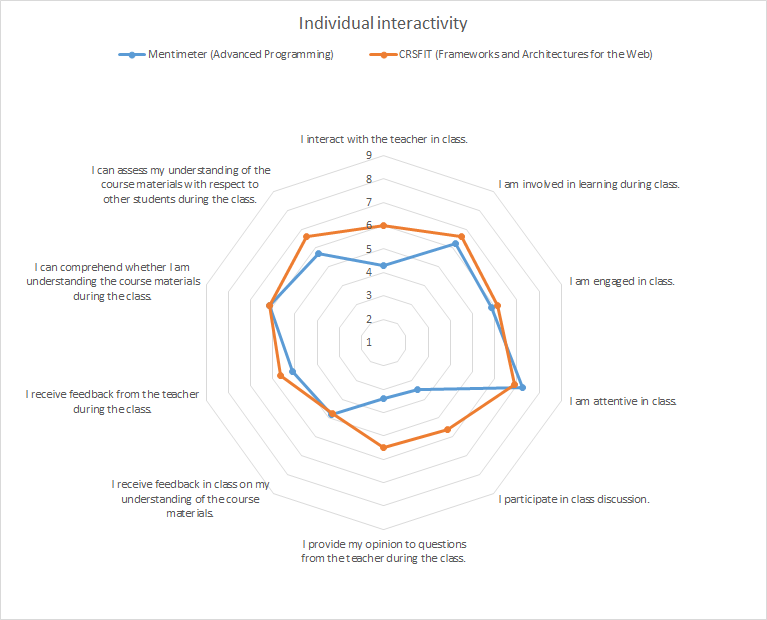
\includegraphics[width=\textwidth]{./individual_interactivity.png}
     \caption{\emph{Pretest - Individual Interactivity.}}
     \label{fig:individual_interactivity}
 \end{figure}

The biggest difference is found in the questions \emph{I participate in class discussion} and \emph{I provide my opinion to questions from the teacher during the class}. These questions are very specific to taking part in class and actively participating, where other questions like \emph{I am involved in learning during class}, might not necessarily imply any direct focus on the individual student. Reasons for these variations could be found in the course differences. Advanced Programming has formal prerequisites where you must be able to program, know basic functional programming, discrete mathematics and more. The Frameworks course is an introductory course so it has no formal prerequisites. Based on this, it is safe to assume that the learning curve is steeper in the Advanced Programming course since it is considered an advanced curriculum, and therefore less people might participate in class discussions since the subjects discussed might be harder to comprehend at first. Also course size might have influenced the outcome. The Advanced Programming course is over twice as large as the Frameworks course (42 vs 89), here students might hold back their participation due to the large amount of people or there simply may not be time to have all students participate.

The responses to the question \emph{I interact with the teacher in class} also has a large difference with a mean of 6 in the Frameworks course versus 4,29 in the Advanced course. Again this outcome can most likely be explained by a larger class and tougher topics that take longer to discuss. It might also involve the teachers style, where some might want to include students more, and some less. A point to notice though, is the fact, that the scores are on each side of the neutral value 5. Where 4,29 is slightly more towards disagreeing and 6 is the other way around.

The general interactivity shows how students think others interact in the course. Compared to the individual interactivity the results here are much more aligned, as mentioned above. The highest differences are found in questions \emph{Students interact with the teacher in class} and \emph{Students are involved in learning during class}, but even here the interval between each is less than 1. We do not find these as a significant difference. Overall the attitude towards general interactivity is very close to each other in both courses. Results for both courses are shown in figure \ref{fig:general_interactivity}.

 \begin{figure}[H]
  \centering
     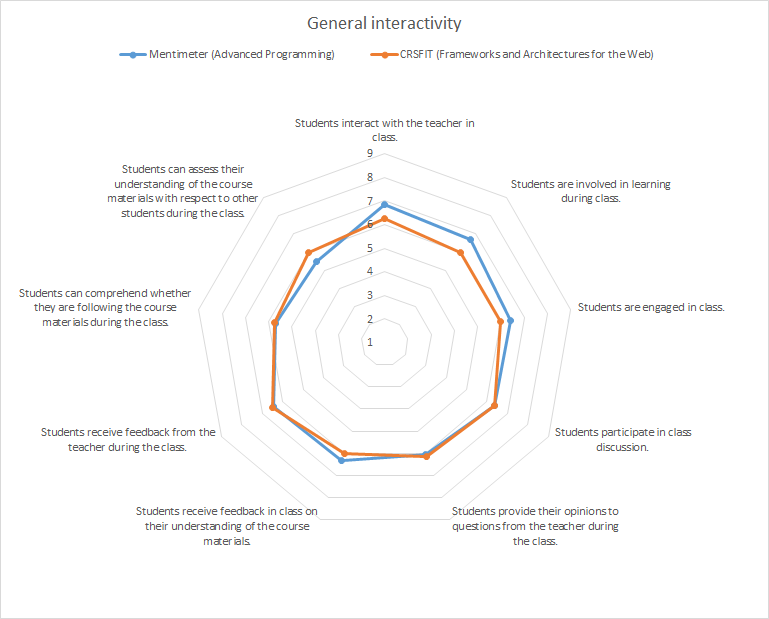
\includegraphics[width=\textwidth]{./general_interactivity.png}
     \caption{\emph{Pretest - General Interactivity.}}
     \label{fig:general_interactivity}
 \end{figure}

Comparing individual and general interactivity on the questions \emph{Students participate in class discussion} and \emph{Students provide their opinions to questions from the teacher during the class}, show that when students are asked to assess themselves, they rate lower, than when asked to assess others. The questions mentioned are the ones with the biggest differences in their answers when asked about individual interactivity but they are exactly the same when asked about general interactivity. This suggest that a small group of people participate in the discussions often, so the general picture is good, but the individual might not be. 



\subsubsection*{Ease of use and perceived usefulness}

% Posttest, mean of Ease of use	and Perceived usefulness
In the posttest we asked the students to assess the \emph{ease of use} and \emph{perceived usefulness} of the CRS they were using. The overall mean of ease of use for CRSFIT is 7,8 and for perceived usefulness it is 6,7, compared to Mentimeters 8,1 and 8,3 respectively, shown in figure \ref{fig:perceived_ease_of_use_and_usefulness}.

 \begin{figure}[H]
  \centering
     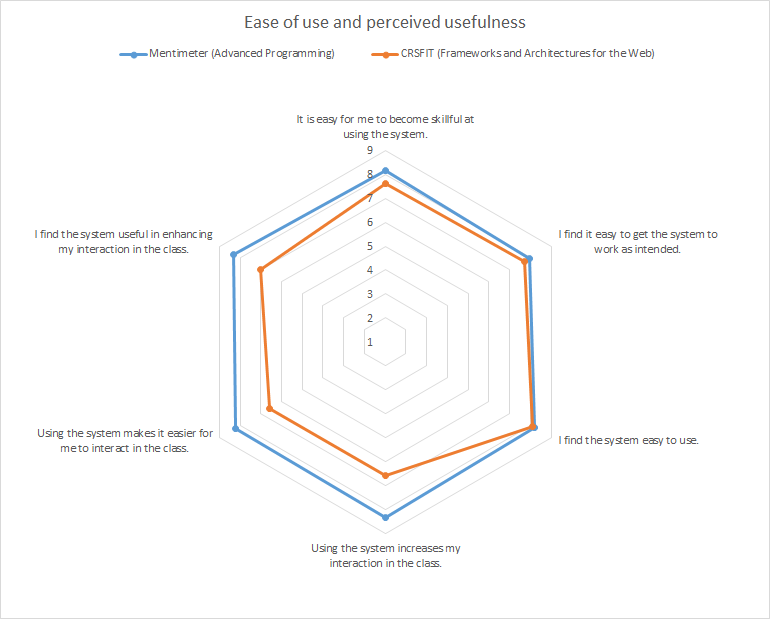
\includegraphics[width=\textwidth]{./perceived_ease_of_use_and_usefulness.png}
     \caption{\emph{Posttest - Ease of use and perceived usefulness.}}
     \label{fig:perceived_ease_of_use_and_usefulness}
 \end{figure}
 
The relatively high value of ease of use suggests that the students found CRSFIT easy to use to an extend that is closely comparable to Mentimeter. The lower level of perceived usefulness could be explained by the way the test was carried out. The results may have been different if the test was carried out over a longer period of time during regular lectures. For example, students might be more convinced that a CRS is useful if they have used it over the course of a whole semester, and therefore rate the perceived usefulness higher. This is compared to testing CRSFIT in just one lecture, where the system is new to them. As mentioned, the class using Mentimeter have had the chance to get well acquainted with the system before doing our test.

As an addition to the test we asked the students whether or not they ran and tested their solutions for the questions they were asked (appendix \ref{app:posttest-open-ended}, item 2). Both the Advanced and Frameworks course were asked questions which included code. We found that only 16\% of students from the Advanced course answered that they ran the code from the questions while 60\% of the Frameworks course answered that they ran the code from the questions. The result from the Advanced course is surprisingly low considering they have used Mentimeter from the beginning of the semester. However, they may have responded relatively to the lecture in which the test was carried out. At the time the test was carried out, the class has been using the REPL, a interactive command line tool for easily running code, for several months.

%% Måske er kodeformateringen med til at få folk til at teste det af? easily copy paste i super CRSFIT, shitty paste i Mentimeter - - - true! De havde jo måske koden i et slide eller hvad ved jeg. Måske noget de ikke havde åbent på pc'eren.

During the test in the Frameworks course, one person mentioned that question 6 (appendix \ref{app:questions}, item 6) was a math question. The question could be asked in any programming language and is not jQuery specific as many of the other questions. This particular question was designed to force the students to run the code since it otherwise would be hard to figure out the correct answer. At this point in the test, it was proposed that in order to answer the question, the students could simply run the code and get the answer. This could be an explanation why 60\% of the students from the Frameworks course answer that they ran the code from the questions. If it had not been brought up during the test, then fewer students might have answered that they ran the code. Despite being brought up how to answer question 6, one still failed to provide the correct answer.

Another, and maybe very important note on the difference between the two courses on whether or not they ran the code from the questions could be the availability of the code. Mentimeter was used by presenting the questions and answers in a separate slideshow and thus not entered into Mentimeter. If these slideshows weren't available to the students during lectures, then copy-pasting the code into a REPL would not be an option and manually writing the code may be too much an effort in order to answer the questions. CRSFIT, on the other hand, provides the code and is thus easily copy-pasted. This may or may not be an advantage. %diskuter



 
 

% last two questions of the pretest
A relatively large amount of the students answered 5 two the last two questions in the pretest. The questions states: \emph{Students can comprehend whether they are following the course materials during the class} and \emph{Students can assess their understanding of the course materials with respect to other students during the class} (appendix \ref{app:pretest-general}, item 8 and 9). 15 and 16 out of a total of 50 students from the Advanced course answered 5 to these questions. 4 and 4 out of a total of 8 students from the Frameworks course answered 5 to these questions. The large amount of neutral responses could suggest that these could be statements which are difficult to assess. Another explanation could be that these statements are the very last in the pretest and students could be bored at this point and just answer 5 two whatever they are asked to assess. Or it could be that a relatively large amount of the students have a neutral opinion to the statements. Either way, the results stands out from the rest with a relatively large amount of neutral answers.














\subsubsection*{Qualitative part of the test}


In the posttest we asked both students from \emph{Advanced Programming} and \emph{Frameworks and Architectures for the Web} into the advantages and disadvantages of using a classroom response system. While the students from Advanced Programming used Mentimeter their comments must be seen in relation to this. The Advanced Programming course has been using Mentimeter from the very beginning of the semester, so they may have more experience with classroom response systems in general. The overall picture from the comments is that the students from Advanced Programming seems pleased with the system. One student points out a disadvantage when saying \emph{"Disadvange could be that people might not get the help they need during Classes."} (appendix \ref{app:qualitative-advanced}, item 25). If the time using a CRS is taken from helping students, then it's a clear disadvantage. However, it will always be the individual teacher's responsibility to manage the time in the courses they teach. Another student mentions awkward pauses when using Mentimeter (\ref{app:qualitative-advanced}, item 13). This may be the same for every CRS and it depends on how the teacher uses the system.

Among many of the advantages reported by the respondents from Advanced Programming is an increased attention, more interaction (\ref{app:qualitative-advanced}, item 4, 6, 10, 12, 13, 14) and forced thinking with feedback (\ref{app:qualitative-advanced}, item 11, 16, 17, 19, 20, 22). These advantages are just some of the advantages any CRS should provide when used properly. The overall picture from Advanced Programming seem that they found Mentimeter useful, which is also the picture we get when looking at the diagram in Figure \ref{fig:perceived_ease_of_use_and_usefulness}, where they report an average score bigger than 8. This is a better score than the one reported by the students from Frameworks and Architectures for the Web. Their comments somewhat reflect that as well, where they tend to be about the situation in which the test was carried out (\ref{app:qualitative-frameworks}, item 1-4).

As highlighted by some of the respondents in the posttest from Frameworks and Architectures for the Web, there's room for improvement when using CRSFIT. The way the test was carried out didn't resemble a normal lecture. As mentioned earlier in chapter \ref{sec:testingcrs}, teaching and using a CRS requires training and experience. The test of the system was not carried out in a normal lecture by a teacher as it would have been if it was a normal setting. The test was carried out by us, letting people answer one question at a time. Normally, a teacher might ask one or two questions after a period of time or after finishing a subject and not ten questions at a time as it was the case in our test.

Two respondents answer that they would like to wait before seeing what other students answered. As one points out: \emph{"Students are easily biased, and it is hard to not look at what everyone else has answered before answering yourself."} (\ref{app:qualitative-frameworks}, item 4). We will not deny that and we may have seen biased answers in our test. For most questions in the test, the majority answered the correct answer except for the very last question. This particular question was made harder and more comprehensive. See appendix \ref{app:questions} item 10. The question got 8 responses and only two of them were correct. This may be because one of the first to answer answered incorrect and most people just followed along due to the difficulty of the question. So the respondents saying to wait some time before revealing answers would be better may have point. If we waited some time before showing what people answered, we would maybe have seen a more even spread in answers or maybe more correct answers in questions like the last one because students would individually take the time to figure out the answer. 

One respondent points out that the system de-personalizes the connection between teacher and student and another says it results in less individual feedback (\ref{app:qualitative-frameworks}, item 3 and 4). This was correct in our setting. A teacher may go more into detail why one answer is correct and another isn't. Maybe a teacher would ask the students why an answer is (in)correct and use the system to start a discussion. This way the personal connection could be maintained for people who are used to interact in class while people not used to interact in class would be included as well through the system.

One comment states that \emph{"it really helps examining yourself and seeing what you got or didn't get- at real time."} (\ref{app:qualitative-frameworks}, item 1). If students using our system immediately sees this advantage then we've come far. All of our questions were centered around topics covered in the course \emph{Frameworks and Architectures for the Web} in which our test was carried out. All of the questions and answers included code in a few different ways and we aimed at asking questions which they should be able to answer if they had followed the course. The comment implies we did that. 


